\documentclass{article}
\usepackage{amssymb}
\usepackage{amsmath}
\usepackage{gastex}
\usepackage{graphicx}

\title{CSE475 Project}
\author{Ben Chavet, Justin McKinstry, Steve Mott}
\date{\today}

\begin{document}
  \maketitle

  \begin{abstract}
    The purpose of this project is to run a simulation with a simple agent
    design, the overarching objective being to achieve coherent behavior
    amongst the agents. The environment is designed to provide a rough
    simulation of how a real fire would spread through a two-dimensional
    area. The firefighter agents are all identical. They are designed to be
    mostly reactive due to the dynamic nature of fighting fires and for
    simplicity of coding. A series of simulations were run with varying numbers
    of firefighters, fires started, and visibility ranges of the firefighters.
    The data is presented in various tables and graphs. Following the
    presentation of the simulation data, observations are made about trends
    and whether the original hypotheses from the beginning of the
    project held true. Justifications for the trends observed follow the
    justifications section, then the implications of these observations are
    presented.
  \end{abstract}

\section{System Design}

  \subsection{Environment}

  The environment in this project consists of an $L \times L$ grid, a maximum
  fire strength, $S_{max}$, a maximum flammability, $F_{max}$, and a maximum
  fuel level, $G_{max}$.  The spaces in the grid are all of equal size, however
  the size is an arbitrary value.  As such, an unlimited number of firefighters are allowed
  to occupy any given space at a time.  Each space in the grid is assigned a random
  flammability value, $F \leq F_{max}$.  This value determines both how
  likely the space is to start on fire, as well as how a fire responds once
  it is started in the space.  This value on each space remains fixed
  throughout the simulation.

  In addition, each space is assigned a random fuel level, $G \leq G_{max}$,
  which is systematically consumed as a fire burns on the space.  At every
  tick, $n$, in the simulation, each space, $i$, in the environment is examined and
  its fire strength, $S_i$, and fuel level, $G_i$, are updated.

  \begin{equation} \label{firestrength}
    S_{i_n} =
    \begin{cases}
      0 & \text{if $S_{i_{n-1}} = 0$, and $\sum{S_{i_{neighbors}}} < F_{max} - F_i$} \\
      1 & \text{if $S_{i_{n-1}} = 0$, $\sum{S_{i_{neighbors}}} \geq F_{max} - F_i$,} \\
        & \text{and a random probability of $P$} \\
      S_{i_{n-1}} + \frac{{F_i}^2}{F_{max}} & \text{if $S_{i_{n-1}} > 0$, $S_{i_{n-1}} < S_{max}$, and $G_{i_{n-1}} > 0$} \\
      S_{max} & \text{if $S_{i_{n-1}} \geq S_{max}$} \\
      S_{i_{n-1}} - \frac{{F_i}^2}{F_{max}} & \text{if $S_{i_{n-1}} > 0$, and $G_{i_{n-1}} = 0$} \\
      S_{i_{n-1}} + 1 & \text{if $S_{i_{n-1}} < 0$} \\
    \end{cases}
  \end{equation}

  \begin{equation} \label{fuellevel}
    G_{i_n} =
    \begin{cases}
      G_{i_{n-1}} & \text{if $S_{i_{n-1}} \leq 0$} \\
      G_{i_{n-1}} - \frac{S_{i_{n-1}}}{S_{max}} & \text{if $S_{i_{n-1}} > 0$} \\
    \end{cases}
  \end{equation}

  These equations are ultimately what control the state of the environment.
  Once a space starts on fire, it can only affect its immediate neighbors
  (not counting diagonals).  This is how a fire is able to spread across the
  environment.

  \subsubsection*{Ignition}

  At each tick, any space can have a fire ignited if there is no fire already present,
  there is still fuel, and the sum of the fire strength of all of the space's
  neighbors is higher than $F_{max} - F_i$, where $F_i$ is the flammability
  level of the space.  Once these conditions are met,
  the chances of a fire igniting are determined by the ignition probability
  variable, $P$.  If a fire is to be started, $S_i$ is set to $1$
  (Eq. \ref{firestrength}).

  This model allows for a space with a high flammability value to
  ignite more readily than a space with a low flammability.  In other words,
  a space with a low flammability requires its neighbors to have a higher
  total fire strength in order to ignite.

  \subsubsection*{Fire Lifespan}

  Once a space is on fire, the strength of that fire increases at every tick
  until either the maximum fire strength, $S_{max}$, is reached or until the
  fuel level of that space, $G_i$, reaches zero.  The number of ticks needed
  for a fire to reach $S_{max}$ depends on the flammability, $F_i$, of the
  space.  A fire on a space with a higher flammability grows faster than a
  fire on a space with a lower flammability (Eq. \ref{firestrength}).

  If a fire's strength, $S_i$, reaches the maximum fire strength, $S_{max}$, it
  remains there until either the fuel level of the space, $G_i$, reaches zero,
  or the fire strength, $S_i$, is reduced due to being sprayed by a
  firefighter agent.  Once the fuel level, $G_i$, reaches zero, the fire starts
  to burn out at the same rate that it grew when it ignited
  (Eq. \ref{firestrength}).

  When $S_i \leq 0$, the fire has been extinguished.  If the fire is
  extinguished due to burning out its fuel, there is no chance of a new fire
  re-igniting on the space.  If the fire was extinguished by a firefighter,
  and there is still fuel in that space ($G_i > 0$), a new fire can still be
  re-ignited in that space.  Also, if a fire is extinguished by a firefighter,
  $S_i$ can be less than zero.  This indicates that the space is wet, and needs
  to dry before it can be re-ignited. Once $S_i = 0$, it remains there until the
  space re-ignites (Eq \ref{firestrength}).

  \subsubsection*{Fuel Consumption}

  As a fire burns on a space, $i$, it consumes the fuel in that space, $G_i$.
  How quickly the fuel burns depends on how strong the fire is, $S_i$
  (Eq. \ref{fuellevel}).  Once the fuel level of a space reaches zero, a fire
  in that space begins to die down.  Once the fire dies, the space is not able
  re-ignite.

  Due to a glitch in the program that was not caught in time, $G_i$ can become
  negative.  This occurs every time that a fire burns itself out, because it
  does not start the burn-out process until $G_i$ already equals zero.  So,
  for every step that the fire is burning out, $G_i$ becomes more negative.
  Fortunately, due to the large amount of total fuel in the environment, this
  glitch is not believed to have significantly changed the outcome of the
  experiments.

  \subsection{Firefighter Agents}

  The firefighter agents are designed to be as autonomous as possible while
  achieving coherent behavior.  In order to achieve this, the logic required
  to make a firefighter able to maximize his well-being was designed first.
  Then, the blackboard communication protocol was designed to allow the
  firefighters to inform each other of the locations of new fires.

  \subsubsection*{Intelligent Design}

  The firefighters were designed to be reactive agents in order to keep the
  design simple.  The only history that a firefighter stores is the locations
  he has visited for the purpose of navigating through the environment towards
  a task.  For all other information, the firefighter just makes observations of the
  environment.

  A firefighter is allowed to move one space and shoot at one space in each
  step.  He can only shoot the space he occupies or a space immediately
  adjacent to that space.  The decision to allow two actions per step was
  justified by arguing that there is no reason that a real firefighter would
  not be able to shoot and move simultaneously.

  With this restriction in mind, a firefighter goes through a series of
  decisions to determine the best course of action at each step (See
  Figure \ref{fig:decisiontree}):

\begin{figure}[htp]
  \centering
  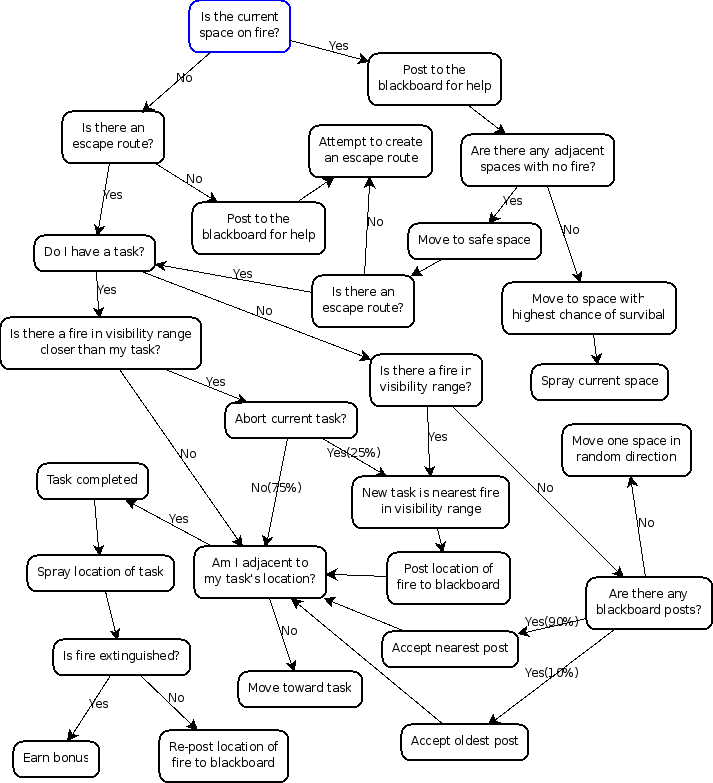
\includegraphics[width=120mm]{images/decisiontree.png}
  \caption{Firefighter Decision Tree}\label{fig:decisiontree}
\end{figure}

  \begin{description}
  \item \textbf{Decision 1:}
    A firefighter first tests to see whether the space he currently  occupies is on
    fire. If it is not on fire, the firefighter can move on to another
    problem, but if it is on fire, he must determine the best course of
    action to minimize the amount of damage received, and ultimately, to keep
    himself alive.

    \begin{description}

    \item{Staying Alive: Part 1}

        It is assumed that a space with no fire is safer than a space
        with fire. It is also assumed that a space with a lower flammability
        is safer than a space with higher flammability. A firefighter takes these
        two assumptions into account when he finds himself on a space that is
        on fire, and is trying to decide the best course of action.  He first
        checks all of the spaces immediately adjacent to the space he currently
        occupies, and if there are one or more that are not on fire, he moves
        to the one that has the lowest flammability.  Once he is in a safe
        location, he then moves on to decide which space to shoot.

    \item{Staying Alive: Part 2}

        If a firefighter is completely surrounded by fire, and the space he
        currently occupies is also on fire, his top priority is to get to the
        safest space.  The safest space is considered to be the space that will
        cause the least amount of damage to the firefighter.

        In this situation, the first thing he does is estimate how strong he
        believes the fire will be at each adjacent space in the next tick.
        This estimation is done based on the current fire strength, the
        flammability, and the amount of fuel on each of these spaces.  The
        space with the lowest result is considered to be the safest.

        Once the safest space has been determined, the firefighter moves to
        that space and immediately shoots it.  By doing so, he is not only
        moving to the space that will cause the least amount of damage, but
        he is also reducing that amount of damage by weakening the fire there.

    \end{description}

  \item \textbf{Decision 2:}
    In an attempt to prevent ever having to act on the first decision, the
    firefighter always looks for an escape route. An escape route is simply an
    adjacent space that is currently not on fire. This means that the firefighter
    has somewhere to move to if the space he occupies starts on fire. If the
    firefighter finds such a space, he moves on to the next decision point,
    otherwise the firefighter finds the adjacent space that will be easiest
    to reduce the fire strength to zero of and shoots it.

  \item \textbf{Decision 3:}
    After a firefighter ensures that he is not on fire and has an escape route,
    he tries to find a fire to extinguish. First, he checks to see if there is
    a fire within visibility range. Then, if he has already accepted a blackboard
    post that is farther away than the fire he spotted, he must choose whether
    to continue toward his task, or to abort and move toward the fire.  This
    decision is based on a random probability, where there is a 75\% chance that
    he will continue toward his task, and a 25\% chance that he will abort
    and move toward the fire.

    If a firefighter does not have a task at hand and there is no visible fire,
    he checks the blackboard for new posts.  While searching the blackboard,
    only the tasks that a firefighter is capable of helping with are considered.
    That is, if a firefighter has low energy, he will not accept a post for a
    fire that has a high intensity.  Also, among the tasks being considered,
    there is a 90\% chance that he will accept the task that is closest to his
    current location, and a 10\% chance that he will accept the oldest post on
    the blackboard.

    If there are no posts on the blackboard, and there are no fires in his
    visibility range, a firefighter chooses a random direction to move.

  \end{description}

  \subsubsection*{Communication}
  The firefighters are capable of communicating with each other by means of a
  simple blackboard system.  The messages that are posted to the blackboard
  simply contain coordinates, and the strength of the fire there, if it is
  known.  The blackboard maintains the messages in the order that they are
  received.  Also, when a response to a message is received, that message is
  removed from the blackboard to prevent multiple responses to a message.

  A firefighter posts a message to the blackboard in various situations.
  Every time a firefighter finds a fire, and decides to move toward it, he posts
  the location and intensity of the fire.  If a firefighter finds himself
  on a space that is on fire, he posts a message to the board, essentially
  asking for help.  Likewise, if a firefighter ever finds himself without an
  immediate escape route, he posts to the board for help.

  A firefighter checks the blackboard when he does not have a task, and there
  are no fires in his visibility range.  While searching the blackboard, there
  is a 90\% chance that the firefighter will choose to respond to the message
  with the closest coordinates to his current location, and a 10\% chance
  that he will choose to respond to the oldest message on the board.

  The purpose of the blackboard system is to help the firefighters find fire
  when they do not have an immediate task to take care of. Because of this,
  it is safe to say that local decision-making is preserved. To ensure the
  firefighters keep their autonomy, they still search for fires on their
  approach to the location of the task they remove from the blackboard. If
  a fire is found closer to the firefighter than the location of the task,
  there is a 25\% chance that the firefighter will abandon the task taken
  from the blackboard to extinguish the closer fire.

  \subsubsection*{Learning}
  The firefighters are not capable of any form of advanced learning.  That is,
  they do not make any decisions based on anything they have encountered in
  the past.  However, when a firefighter earns the bonus from extinguishing
  a fire, that bonus is then applied to how well a firefighter can fight the
  next fire.  So, as a firefighter extinguishes more fires, he is able to put
  out later fires with greater ease.  While this is not technically
  ``learning'' in a MAS point of view, it is quite obvious that the
  firefighters are quicker to put out fires later in the simulation.

  \subsection{Definitions}
  \begin{description}
    \item \textbf{Effectiveness:}
      The effectiveness of the system is measured by comparing the percentage of
      fuel remaining in the environment at the end of the simulation against the
      baseline percentage of fuel remaining after running the simulation with no
      firefighters.  If the percentage is higher than the baseline, the system
      is considered to be effective.  The higher the percentage, the more
      effective the system is.

    \item \textbf{Efficiency:}
      The efficiency of the system is determined by the total amount of firefighter
      health remaining at the end of a simulation.  If the total amount of health
      reaches zero, that means that all of the firefighters were killed, and the
      system is not considered to be efficient at all.

    \item \textbf{Coherence:}
      The system is considered to reach coherence if both effectiveness and
      efficiency are reached on some level.  That is, at least one firefighter
      must survive, and the remaining fuel level must be higher than what it
      would have been if there were no firefighters.

  \end{description}

  \subsection{Hypotheses}

  \begin{description}

  \item \textbf{Hypothesis 1:}
    The effectiveness of the team of firefighter agents is proportional to
    $\frac{N}{K}$.  However, if $N \ll K$, then the effectiveness becomes
    non-existent, and the fire will end up burning up most of the available
    fuel in the environment.

  \item \textbf{Hypothesis 2:}
    The efficiency of the team of firefighter agents is proportional to
    $\frac{N}{K}$.  However, if $N \ll K$, then the efficiency becomes
    non-existent, and the firefighters are all likely to be killed.

  \item \textbf{Hypothesis 3:}
    If $L \times L \gg N$ and $K \gg N$, then the system will not achieve
    coherence.  On the other hand, if $N \approxeq L \times L$ and $N \gg K$,
    then the system will achieve coherence quickly.

  \item \textbf{Hypothesis 4:}
    The effectiveness of the system is proportional to $V$.  That is,
    the farther a firefighter can see in the environment, the better the
    chances are that he will see a previously undetected fire, and thus
    yielding a higher overall effectiveness for the system.

  \item \textbf{Hypothesis 5:}
    The chances of one or more firefighter agents becoming a ``super-agent''
    is directly proportional to $K$.  A ``super-agent'' is a firefighter agent
    an energy level that is higher than the maximum allowed fire strength, thus
    allowing that firefighter to extinguish any fire in the environment in one shot.
    If there are more initial fires in the environment, there are more chances
    for one or more agents to put out enough fires to earn ``super-agent''
    status.

  \end{description}

\section{Presentation}

  The experiments were designed to test each of the above hypotheses by
  adjusting key parameters as shown in Table \ref{tab:experiments}. 
  Thirty-two simulations were run for each possible combination of the
  values shown in order to maintain statistic validity.

\begin{table}[htp]
  \caption{Experiments}
  \label{tab:experiments}
  \centerline{
  \begin{tabular}{ | l | l | l | }
    \hline
    {\bf Parameter} & {\bf Variable} & {\bf Range of Values} \\
    \hline
    Grid size & $L$ & 100 \\
    \hline
    Number of firefighter agents & $N$ & 0, 10, 50, 100, 500 \\
    \hline
    Number of fires started & $K$ & 1, 5, 10, 500 \\
    \hline
    Firefighters' visibility range & $V$ & 1, 15, 50 \\
    \hline
  \end{tabular}}
\end{table}

\begin{description}
  \item \textbf{Hypothesis 1:}
    Hypothesis 1 required testing the effectiveness of the system for various
    values of $N$ and $K$.  Table \ref{tab:effectiveness} and Figure
    \ref{fig:effectiveness} show the results of these tests.

    \begin{figure}[htp]
      \centering
      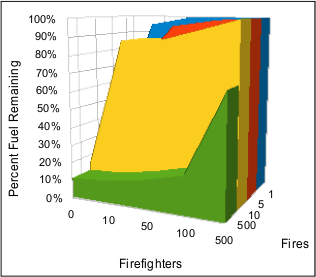
\includegraphics[width=60mm]{images/effectiveness1.png}
      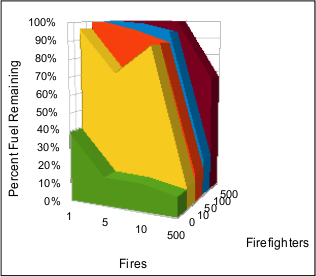
\includegraphics[width=60mm]{images/effectiveness2.png}
      \caption{System Effectiveness}\label{fig:effectiveness}
    \end{figure}

    \begin{table}[htp]
      \caption{System Effectiveness}
      \label{tab:effectiveness}
      \centerline{
      \begin{tabular}{ | r | r | r | }
        \hline
        {\bf Fires} & {\bf Firefighters} & {\bf Percent Fuel Remaining} \\
        \hline
        1 & 0 & 39.66\% \\
        \hline
        1 & 10 & 95.98\% \\
        \hline
        1 & 50 & 99.80\% \\
        \hline
        1 & 100 & 99.94\% \\
        \hline
        1 & 500 & 99.99\% \\
        \hline
        5 & 0 & 15.88\% \\
        \hline
        5 & 10 & 72.34\% \\
        \hline
        5 & 50 & 95.17\% \\
        \hline
        5 & 100 & 98.61\% \\
        \hline
        5 & 500 & 99.97\% \\
        \hline
        10 & 0 & 15.35\% \\
        \hline
        10 & 10 & 87.84\% \\
        \hline
        10 & 50 & 88.46\% \\
        \hline
        10 & 100 & 93.97\% \\
        \hline
        10 & 500 & 99.93\% \\
        \hline
        500 & 0 & 11.17\% \\
        \hline
        500 & 10 & 12.21\% \\
        \hline
        500 & 50 & 16.19\% \\
        \hline
        500 & 100 & 21.52\% \\
        \hline
        500 & 500 & 66.90\% \\
        \hline
      \end{tabular}}
    \end{table}

  \item \textbf{Hypothesis 2:}
    Hypothesis 2 required testing the efficiency of the system for various
    values of $N$ and $K$.  Table \ref{tab:efficiency} and Figure
    \ref{fig:efficiency} show the results of these tests.

    \begin{figure}[htp]
      \centering
      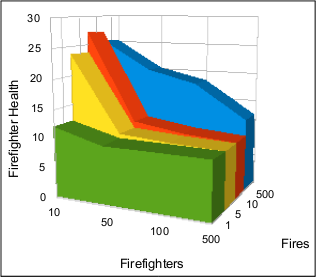
\includegraphics[width=60mm]{images/efficiency.png}
      \caption{System Efficiency}\label{fig:efficiency}
    \end{figure}

    \begin{table}[htp]
      \caption{System Efficiency}
      \label{tab:efficiency}
      \centerline{
      \begin{tabular}{ | r | r | r | }
        \hline
        {\bf Fires} & {\bf Firefighters} & {\bf Firefighter Health} \\
        \hline
        1 & 10 & 12.16 \\
        \hline
        1 & 50 & 9.82 \\
        \hline
        1 & 100 & 9.73 \\
        \hline
        1 & 500 & 9.7 \\
        \hline
        5 & 10 & 23.77 \\
        \hline
        5 & 50 & 10.66 \\
        \hline
        5 & 100 & 9.94 \\
        \hline
        5 & 500 & 9.71 \\
        \hline
        10 & 10 & 27.22 \\
        \hline
        10 & 50 & 11.68 \\
        \hline
        10 & 100 & 10.36 \\
        \hline
        10 & 500 & 9.72 \\
        \hline
        500 & 10 & 25.41 \\
        \hline
        500 & 50 & 20.34 \\
        \hline
        500 & 100 & 18.35 \\
        \hline
        500 & 500 & 12.54 \\
        \hline
      \end{tabular}}
    \end{table}

  \item \textbf{Hypothesis 3:}
    Hypothesis 3 required testing both the efficiency and effectiveness of the
    system for extreme values of $N$ and $K$, such that $N \gg K$, or $N \ll K$.
    Tables \ref{tab:effectiveness} and \ref{tab:efficiency} as well as Figures
    \ref{fig:nltk} and \ref{fig:ngtk} show the results of these tests.

    \begin{figure}[htp]
      \centering
      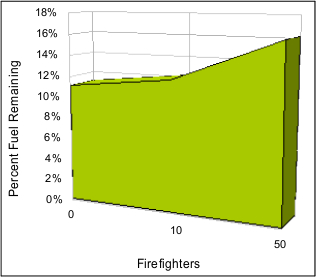
\includegraphics[width=60mm]{images/k500.png}
      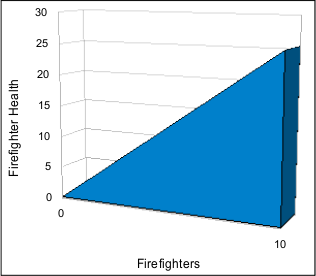
\includegraphics[width=60mm]{images/k500efficiency.png}
      \caption{System Convergence when $K \gg N$ ($K = 500$)}\label{fig:nltk}
    \end{figure}

    \begin{figure}[htp]
      \centering
      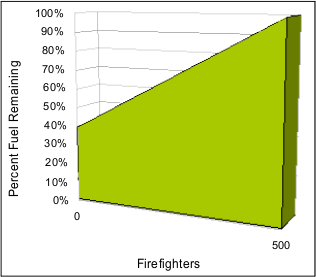
\includegraphics[width=60mm]{images/k1.png}
      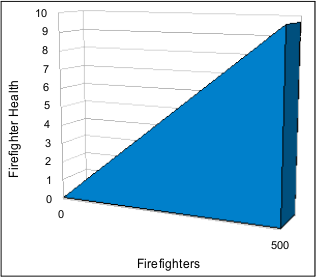
\includegraphics[width=60mm]{images/k1efficiency.png}
      \caption{System Convergence when $N \gg K$ ($K = 1$)}\label{fig:ngtk}
    \end{figure}

  \item \textbf{Hypothesis 4:}
    Hypothesis 4 required testing the effectiveness of the system for various
    values of $V$.  Table \ref{tab:visibility} and Figure \ref{fig:visibility}
    show the results of these tests.

    \begin{figure}[htp]
      \centering
      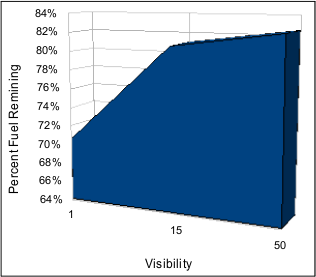
\includegraphics[width=60mm]{images/visibility.png}
      \caption{Visibility}\label{fig:visibility}
    \end{figure}

    \begin{table}[htp]
      \caption{Visibility}
      \label{tab:visibility}
      \centerline{
      \begin{tabular}{ | r | r | }
        \hline
        {\bf Visibility} & {\bf Percent Fuel Remaining} \\
        \hline
        1 & 70.65\% \\
        \hline
        15 & 81.01\% \\
        \hline
        50 & 82.50\% \\
        \hline
      \end{tabular}}
    \end{table}

  \item \textbf{Hypothesis 5:}
    Hypothesis 5 required checking for the regular emergence of ``super-agents.''
    While there were instances of ``super-agents'' in the raw data, the were
    very isolated.

\end{description}


\section{Observations}

  \begin{description}

    \item \textbf{Hypothesis 1:}
      According to the experimental data, this hypothesis is shown to be true.  The
      effectiveness of the team of firefighters is proportional to $\frac{N}{K}$.
      That is, if there are more firefighters than there are fires, the system
      is more effective.  The converse is also true, if there are more fires than
      there are firefighters, then the system is less effective.  It also holds
      that if $N \ll K$, the effectiveness becomes nearly non-existent, and the
      fire burns approximately the same amount of fuel as if there were no
      firefighters to begin with.

    \item \textbf{Hypothesis 2:}
      According to the experimental data, this hypothesis does not hold.  Instead, the
      opposite is true.  The efficiency is actually inversely proportional to
      $\frac{N}{K}$.  That is, if there are more firefighters than there are
      fires, the system is \textit{less} efficient.  The converse is also true, if
      there are more fires than there are firefighters, the system is \textit{more}
      efficient.  Also, if $N \ll K$, the system still retains a certain amount
      of efficiency.

    \item \textbf{Hypothesis 3:}
      According to the experimental data, the system achieves coherence,
      regardless of the relationship between $L \times L$, $N$, and $K$.
      That is, in no instance did all of the firefighters die during a
      simulation.  Therefore, coherence was always achieved at some level.

      On the other hand, when $N \approxeq L \times L$ and $N \gg K$,
      the system did achieve coherence very quickly.

    \item \textbf{Hypothesis 4:}
      According to the experimental data, the effectiveness of the system is
      proportional to $V$.  That is, the farther the firefighters can see in
      the environment, the more effective the system is.

    \item \textbf{Hypothesis 5:}
      There are instances when one or more ``super-agent'' emerges during a
      simulation.  However, it does not happen frequently enough to conclusively
      determine whether it is proportional to $K$.

  \end{description}

\section{Justifications}

  \begin{description}

    \item \textbf{Hypothesis 1:}
      Recall that the effectiveness of the system is measured by the percentage
      of total fuel remaining in the environment.  So, when there are more
      firefighters, the firefighters are more likely to find a fire more quickly.
      In doing so, the other firefighters are then notified of the location
      of that fire, and the more firefighters there are, the more likely there
      are firefighters that do not have a task that can respond to the new fire
      notification.  More firefighters that are fighting a given fire results
      in the fire being extinguished more quickly, resulting in a higher amount
      of fuel remaining at the space that the fire was.  Multiplied over the
      space of the environment, this yields a higher overall effectiveness.

      Likewise, when there are more fires, the effectiveness of the system
      is lower.  Even though the firefighters are more likely to find a fire
      if there are more of them throughout the environment, they are not
      able to keep up with the fire, and it ends up burning more of the
      fuel in the environment.

    \item \textbf{Hypothesis 2:}
      Recall that the efficiency of the system is determined by the total amount
      of firefighter health after a simulation.  Due to the design of the
      firefighter agents, when they find themselves in a situation that reduces
      their health, they are very good at choosing the action that minimizes
      how much their health is reduced.  Because of this, the firefighters are
      able to be very aggressive when they find a fire.  Therefore, when there are
      more fires, there are more opportunities to earn the bonus from extinguishing
      a fire.  This leads to a higher overall efficiency when there are more
      fires.

      This is different than what was hypothesized.  It was thought that when
      there were more fires, the firefighters would be more likely to be
      injured or killed, thus reducing the overall efficiency.  However, the
      ability of the firefighters to minimize the amount of damage they
      receive from being in a bad situation was not taken well enough into
      account.

    \item \textbf{Hypothesis 3:}
      The fact that coherence is always achieved can also be accounted to the
      design of the firefighter agents.  The decisions that are made to
      minimize the amount of damage taken lead to agents being very good at
      surviving even the worst scenarios.

      As expected, when there are many more firefighters than there
      are fires, the system converges very quickly.  This is due to the fact
      that the firefighters cover much of the environment, and are likely to
      locate the fire(s) very quickly.  Also, when a fire is located, there
      is a larger number of firefighters that are not very far away. Thus,
      they are able to respond very quickly, resulting in a very rapid convergence.

    \item \textbf{Hypothesis 4:}
      Again, recall that the effectiveness of the system is determined by the
      total amount of fuel remaining in the environment after the simulation.
      The farther a firefighter is able to see, the more likely he is to locate
      a previously undetected fire, and move towards it.  When the firefighters
      were not given any visibility range, they would wander aimlessly, even
      if there was a fire two spaces away.  They simply could not see it, so it
      was allowed to burn, resulting in a lower effectiveness.  When the fire
      can be more easily detected, the overall effectiveness of the system
      is higher.

    \item \textbf{Hypothesis 5:}
      Recall that the definition of a ``super-agent'' is a firefighter agent
      that achieves a health level that is higher than the maximum allowed
      fire strength, thus allowing the firefighter to easily extinguish any
      fire in one step.  While ``super-agents'' did emerge on occasion, the
      lack of consistency is believed to be due to the iterative nature of the
      simulations as well as the reward system only rewarding the firefighter
      that actually extinguishes the fire.  That is, there can be multiple
      firefighters in the same location fighting the same fire, but only the
      firefighter that extinguishes the fire earns the bonus health point.
      This leads to a fairly even distribution of the bonus health points
      which actually reduces the chances of the emergence of a ``super-agent.''

  \end{description}

\section{Implications}

  \begin{description}
    \item \textbf{Hypothesis 1:}
      As shown, hypothesis 1 proved to be true. This means that when designing
      a system, in order to make it as effective as possible, the designer
      should be sure to make the ratio of firefighters to initial fires as
      high as possible.

    \item \textbf{Hypothesis 2:}
      The results of this hypothesis indicate two errors in the design and
      implementation of the firefighter agents.

      The first is that the firefighters were made to be too competitive.
      This was not in the intention of the design.  It originally did not
      appear that there was anything to compete over. The problem is that
      only the firefighter that extinguishes a fire gets the energy reward.
      This means that all of the other firefighters that were helping
      fight the fire do not receive any reward for helping.

      Part of the reason for this competition is because of the nature of
      Repast. Since Repast iterates through the steps of each agent, the
      agents are not actually spraying the fire at the same time (which is
      what the simulation intends). If there were a way to run a multi-threaded
      version of the simulation, this problem would be minimized.

      The best way to solve this problem, is to reward all agents who
      actively participated in extinguishing the fire, and were present at
      the time the fire was extinguished. Although this solution still does
      not allow for the agents to all be spraying at the same time, it provides
      a logical method of rewarding the firefighters as though they were all
      working together in real time.

      If the reward problem is not solved, this presents an interesting
      dilemma for the design of future simulations. A higher ratio of
      firefighters to fires means fewer firefighters are going to be
      able to receive energy bonuses, and the average firefighter energy will
      be low, meaning the efficiency of the system will suffer.
      However, as previously noted, using a higher ratio means the
      firefighters are more effective.

      This is a delicate balance that needs to be chosen appropriately for the
      type of simulation being run. If the firefighters need to maximize their
      energy, a low ratio should be chosen, while a high ratio should be chosen
      if the fire needs to be put out quickly with little damage done to the
      environment.

    \item \textbf{Hypothesis 3:}
      The firefighter design works very well. The firefighters seem to have a
      very good balance between teamwork and self interest in order to keep
      everyone alive while extinguishing the fire in a timely manner. The
      next step for making the firefighters more intelligent would be to
      add a way for them to learn and plan. If the firefighters were able
      to recognize areas of low flammability, or low fuel levels, they could
      plan on retreating back to that place if they get overwhelmed with fire.
      They could also communicate with each other so that they can share their
      ``safe zones'' so that they can team up and conquer the fire in an
      organized manner.

      These additions would require a more robust communication protocol than
      the blackboard system currently implemented. Some sort of negotiation
      protocol would be needed for the agents to choose the best location to
      set up their ``safe zones.'' They would also require some modifications
      to the way the agents store the maps in their memory. Currently, the
      agents construct a map of spaces they have visited in case they
      get lost in a maze of fire while trying to move toward a call for help.
      This internal map can be modified to store flammability and fuel level
      information so that the firefighter can recognize larger areas of safe
      spaces to suggest as a ``safe zone.''

    \item \textbf{Hypothesis 4:}
      Obviously, a higher visibility leads to a more effective system. The
      only problem is keeping that visibility within a reasonable range. If
      this system is being used to try and model a real fire fighting
      situation, it would be important to use realistic visibility levels.

      In future versions, it would be interesting to make the visibility
      levels of the firefighters a variable value based on a firefighters
      location in the environment. Fires that burn for longer periods of
      time, or fires that have lower flammability would tend to create more
      smoke in the area surrounding them and would cause lower visibility.

    \item \textbf{Hypothesis 5:}
      Assuming ``super-agents'' are desirable, the system can be altered to
      allow for easier emergence of one or more ``super-agents.'' The reasons
      there are only occasional ``super-agents'' are almost the same for the
      reason that the efficiency goes down when more firefighters are added
      to the system.

      This provides more reason to alter the system as outlined in the
      implications for hypothesis 2. The simulation would ideally be run in a
      multi-threaded environment so that the agents can all spray fires
      simultaneously. The system should also assign rewards to agents who are
      actively trying to extinguish the fire at the time that the fire goes out.

  \end{description}

\begin{thebibliography}{1}
\bibitem{bib:markov}
  ``MARKOV LATTICE MODEL OF FIRE SPREAD'', Den Boychuk, MNR Ontario,
  John Braun, Zinovi Krougly, Reg Kulperger, Dave Stanford
\bibitem{bib:devs}
  ``Two-dimensional fire spread decomposition in cellular DEVS models'', Ntaimo,
  L. and Khargharia B., Proceedings of Spring Simulation Multi-Conference,
  Huntsville, AL, April, 2006
\end{thebibliography}

\end{document}
